% ====================================================================
%  徐森林、薛春华《数学分析》（第一册）
%  \S3.1  导数及其运算法则
%  源：原书印刷页 153-171（PDF 物理页 159-177）
%  底本：PaddleOCR-VL-1.6 + 高清影印比对校订
%  规范：全西文半角标点；单一落盘出口 _texout.py
% ====================================================================
\section{导数及其运算法则}\label{sec:3.1}

\begin{example}\label{ex:3.1.1}
设质点作直线运动, 在时刻 $t$ 的位移可用函数 $x = x(t)$ 来描述. 在时间段 $[t, t+\Delta t]$ 中位移的改变量为 $\Delta x = x(t+\Delta t) - x(t)$. 当 $\Delta t$ 很小时, 它在时刻 $t$ 的瞬时速度可近似地用它在 $[t, t+\Delta t]$ 中的平均速度
\[
\overline{v}(t,\Delta t) = \frac{\Delta x}{\Delta t} = \frac{x(t+\Delta t) - x(t)}{\Delta t}
\]
来代替. 如果当 $\Delta t \to 0$ 时, 极限
\[
v(t) = \lim_{\Delta t\to0}\frac{\Delta x}{\Delta t} = \lim_{\Delta t\to0}\frac{x(t+\Delta t) - x(t)}{\Delta t}
\]
存在有限, 则称它为质点在时刻 $t$ 的瞬时速度, 并记为 $v(t) = x'(t)$. 瞬时速度问题是微积分发明人之一——Newton 最早研究的.
\end{example}

\begin{example}\label{ex:3.1.2}
设直细棒从 $0$ 到 $x$ 一段的质量为 $m = m(x)$, 在 $[x, x+\Delta x]$ 一段的质量为 $\Delta m = m(x+\Delta x) - m(x)$. 当 $\Delta x$ 很小时, 在 $x$ 处的线密度可近似地用它在 $[x, x+\Delta x]$ 中的平均线密度
\[
\frac{\Delta m}{\Delta x} = \frac{m(x+\Delta x) - m(x)}{\Delta x}
\]
来代替. 如果当 $\Delta x \to 0$ 时, 极限
\[
\lim_{\Delta x\to0}\frac{\Delta m}{\Delta x} = \lim_{\Delta x\to0}\frac{m(x+\Delta x) - m(x)}{\Delta x}
\]
存在且有限, 则称它为直细棒在点 $x$ 处的线密度, 记为 $m'(x)$.
\end{example}

\begin{example}\label{ex:3.1.3}
设函数 $p = p(t)$ 表示某地区在时刻 $t$ 的人口数目, 则在时刻 $t+\Delta t$ 的人口数目就是 $p(t+\Delta t)$. 因此, 这个地区在从 $t$ 到 $t+\Delta t$ 的时间段中, 人口平均增长速度为
\[
\frac{\Delta p}{\Delta t} = \frac{p(t+\Delta t) - p(t)}{\Delta t}.
\]
如果当 $\Delta t \to 0$ 时, 极限
\[
\lim_{\Delta t\to0}\frac{\Delta p}{\Delta t} = \lim_{\Delta t\to0}\frac{p(t+\Delta t) - p(t)}{\Delta t}
\]
存在且有限, 则称它为该地区在时刻 $t$ 的人口增长速率, 并记为 $p'(t)$.
\end{example}

\begin{example}\label{ex:3.1.4}
设 $(x, f(x))$ 为曲线 $y = f(x)$ 上的一个定点, 而 $(x+\Delta x, f(x+\Delta x))$ 为该曲线上的一个动点. 显然, 通过点 $(x, f(x))$ 与 $(x+\Delta x, f(x+\Delta x))$ 的割线的斜率为
\[
\frac{\Delta y}{\Delta x} = \frac{f(x+\Delta x) - f(x)}{\Delta x},
\]
它是 $[x, x+\Delta x]$ 上函数 $y = f(x)$ 的平均变化率. 如果当 $\Delta x \to 0$ 时, 极限
\[
\lim_{\Delta x\to0}\frac{\Delta y}{\Delta x} = \lim_{\Delta x\to0}\frac{f(x+\Delta x) - f(x)}{\Delta x}
\]
存在且有限, 则称它为函数 $y = f(x)$ 在 $x$ 处的变化率, 记为 $f'(x)$, 并称它为 $f(x)$ 在 $x$ 处的导数. 称过点 $(x, f(x))$ 斜率为 $f'(x)$ 的直线(即割线的极限位置)为该点处的切线. 在图~\ref{fig:3.1.1} 中, $\frac{\Delta y}{\Delta x} = \tan\varphi$, $f'(x) = \lim\limits_{\Delta x\to0}\frac{\Delta y}{\Delta x} = \tan\varphi_0$.

由此进而可得, 曲线 $y = f(x)$ 在点 $(x_0, f(x_0))$ 处的切线方程为
\[
y - f(x_0) = f'(x_0)(x - x_0).
\]
过点 $(x_0, f(x_0))$ 且与切线垂直的直线称为曲线 $y = f(x)$ 在点 $(x_0, f(x_0))$ 处的法线. 于是, 当 $f'(x_0) \neq 0$ 时, 在点 $(x_0, f(x_0))$ 处法线为
\[
y - f(x_0) = -\frac{1}{f'(x_0)}(x - x_0);
\]
当 $f'(x_0) = 0$ 时, 在点 $(x_0, f(x_0))$ 处法线为 $x = x_0$. 两种情形统一表达为
\[
(x - x_0) + f'(x_0)(y - f(x_0)) = 0.
\]
Leibniz 的巨大贡献之一, 就是发现了曲线的切线斜率与函数的导数之间的联系, 同时得到了计算导数的一般方法. 下面来正式引进导数的概念.
\end{example}

\begin{figure}[htbp]
\centering
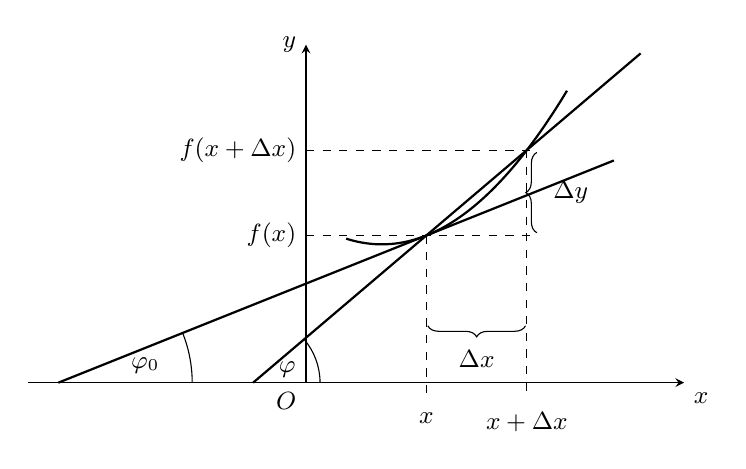
\begin{tikzpicture}[scale=0.85,>=stealth,font=\small]
  % 坐标轴
  \draw[->] (-3.15,0) -- (6.65,0) node[below right] {$x$};
  \draw[->] (1.0,0) -- (1.0,5.05) node[left] {$y$};
  \node[below left] at (1.0,0) {$O$};
  % 曲线 y=f(x)
  \draw[thick] plot[domain=1.6:4.9,samples=60,smooth]
    (\x,{0.30*(\x-2.8)*(\x-2.8)+0.40*(\x-2.8)+2.2});
  % 切线 (过 P(2.8,2.2), 斜率 0.40, 交 x 轴于 (-2.7,0))
  \draw[thick] (-2.7,0) -- (5.6,3.32);
  % 割线 PQ (斜率 0.85, 交 x 轴于 (0.21,0))
  \draw[thick] (0.21,0) -- (6.0,4.92);
  % 虚线
  \draw[dashed] (1.0,2.2) -- (4.45,2.2);
  \draw[dashed] (1.0,3.475) -- (4.45,3.475);
  \draw[dashed] (2.8,2.2) -- (2.8,-0.22);
  \draw[dashed] (4.3,3.475) -- (4.3,-0.22);
  % 纵坐标标注
  \node[left] at (1.0,2.2) {$f(x)$};
  \node[left] at (1.0,3.475) {$f(x+\Delta x)$};
  % 横坐标标注
  \node[below] at (2.8,-0.30) {$x$};
  \node[below] at (4.3,-0.30) {$x+\Delta x$};
  % Delta x 括号
  \draw[decorate,decoration={brace,amplitude=4pt,mirror}]
    (2.82,0.85) -- (4.28,0.85);
  \node at (3.55,0.36) {$\Delta x$};
  % Delta y 括号
  \draw[decorate,decoration={brace,amplitude=4pt}]
    (4.45,2.24) -- (4.45,3.44);
  \node[right] at (4.55,2.84) {$\Delta y$};
  % 角 φ0 (切线与 x 轴夹角)
  \draw (-2.7,0) ++(2.0,0) arc (0:21.8:2.0);
  \node at (-1.40,0.26) {$\varphi_0$};
  % 角 φ (割线与 x 轴夹角)
  \draw (0.21,0) ++(1.0,0) arc (0:40.4:1.0);
  \node at (0.72,0.20) {$\varphi$};
\end{tikzpicture}
\caption{}\label{fig:3.1.1}
\end{figure}

\begin{definition}[导数]\label{def:3.1.1}
设函数 $y = f(x)$ 在点 $x_0$ 处的某开邻域 $(x_0 - \delta_0, x_0 + \delta_0)$ (点 $x_0$ 附近)有定义. 如果极限
\[
\lim_{x\to x_0}\frac{f(x) - f(x_0)}{x - x_0} = \lim_{\Delta x\to0}\frac{f(x_0+\Delta x) - f(x_0)}{\Delta x} = \lim_{\Delta x\to0}\frac{\Delta y}{\Delta x}
\]
存在且有限, 则称函数 $f$ 在点 $x_0$ 处可导, 且称此极限值为 $f$ 在点 $x_0$ 处的导数(或变化率), 记为
\[
f'(x_0)\ \text{或}\ f'(x)|_{x=x_0}\ \text{或}\ \frac{\mathrm{d}f}{\mathrm{d}x}\Big|_{x=x_0}\ \text{或}\ y'(x_0)\ \text{或}\ \frac{\mathrm{d}y}{\mathrm{d}x}\Big|_{x=x_0},
\]
其中, $\Delta x = x - x_0$ 称为自变量 $x$ 的增量, 而 $\Delta y = f(x_0+\Delta x) - f(x_0)$ 称为函数(因变量)$y$ 的增量, $\frac{\Delta y}{\Delta x}$ 称为平均变化率.
\end{definition}

由定义~\ref{def:3.1.1} 知, 瞬时速度就是质点作直线运动的位移函数 $x(t)$ 对时间 $t$ 的导数; 直细棒的线密度就是其质量函数 $m(x)$ 对 $x$ 的导数, 这就是导数的物理意义. 切线的斜率就是 $y = f(x)$ 对 $x$ 的导数, 这是导数的几何意义.

用"$\varepsilon$-$\delta$"语言描述导数如下: $\forall \varepsilon > 0, \exists \delta > 0$, 当 $0 < |x - x_0| < \delta$ 时,
\[
\left|\frac{f(x) - f(x_0)}{x - x_0} - f'(x_0)\right| < \varepsilon,
\]
\[
\left|\frac{f(x_0+\Delta x) - f(x_0)}{\Delta x} - f'(x_0)\right| < \varepsilon.
\]

设 $f$ 在点 $x_0$ 的左旁 $(x_0 - \delta_0, x_0]$ 有定义, 如果
\[
\lim_{x\to x_0^-}\frac{f(x) - f(x_0)}{x - x_0} = \lim_{\Delta x\to0^-}\frac{f(x_0+\Delta x) - f(x_0)}{\Delta x}
\]
存在且有限, 则称此极限值为 $f$ 在点 $x_0$ 处的左导数, 记为 $f'_-(x_0)$. 类似可定义 $f$ 在点 $x_0$ 处的右导数 $f'_+(x_0)$.

\begin{theorem}\label{thm:3.1.1}
$f$ 在点 $x_0$ 处可导 $\iff f$ 在点 $x_0$ 处既左可导又右可导, 且 $f'_-(x_0) = f'_+(x_0)$.
\end{theorem}

\begin{proof}
$f$ 在点 $x_0$ 处可导, 即
\[
\lim_{x\to x_0}\frac{f(x) - f(x_0)}{x - x_0} = f'(x_0) \in \mathbb{R}
\]
\[
\iff f'_-(x_0) = \lim_{x\to x_0^-}\frac{f(x) - f(x_0)}{x - x_0} = \lim_{x\to x_0^+}\frac{f(x) - f(x_0)}{x - x_0} = f'_+(x_0) \in \mathbb{R},
\]
且 $f'_-(x_0) = f'(x_0) = f'_+(x_0)$.
\end{proof}

\begin{definition}\label{def:3.1.2}
如果 $y = f(x)$ 在开区间 $(a,b)$ 内的任一点 $x$ 处可导, 则称 $f$ 在 $(a,b)$ 内可导; 如果 $f$ 在有界区间 $(a,b)$ 内可导, 又在 $a$ 处右可导, 在 $b$ 处左可导, 则称 $f$ 在闭区间 $[a,b]$ 上可导.
\end{definition}

$f(x)$ 在区间 $I$ 中的导数形成一个新函数 $f'(x)$, 称为 $f(x)$ 的导函数. 如果 $f'(x)$ 为 $I$ 上的连续函数, 即 $\lim\limits_{x\to x_0}f'(x) = f'(x_0)$, $\forall x_0 \in I$, 则称 $f$ 为 $1$ 阶连续可导的函数.

注意, $f'_-(x_0)$ ($f'_+(x_0)$)为 $f$ 在点 $x_0$ 处的左(右)导数, 但是 $f'(x_0^-) = \lim\limits_{x\to x_0^-}f'(x)$ ($f'(x_0^+) = \lim\limits_{x\to x_0^+}f'(x)$)为导函数 $f'(x)$ 在点 $x_0$ 处的左(右)极限.

\begin{theorem}\label{thm:3.1.2}
设 $f$ 在点 $x_0$ 处可导, 则 $f$ 在点 $x_0$ 处连续. 反之不真.
\end{theorem}

\begin{proof}
($\Rightarrow$) 设 $f$ 在点 $x_0$ 处可导, 则
\[
\lim_{x\to x_0}f(x) = \lim_{x\to x_0}\left[\frac{f(x) - f(x_0)}{x - x_0}(x - x_0) + f(x_0)\right] = f'(x_0)\cdot0 + f(x_0) = f(x_0).
\]
这就证明了 $f$ 在点 $x_0$ 处连续.

($\Leftarrow$) 反例: $f(x) = |x|$ 在 $x_0 = 0$ 处连续, 但在 $x_0 = 0$ 处不可导.

事实上, 由
\[
f'_+(0) = \lim_{x\to0^+}\frac{f(x) - f(0)}{x - 0} = \lim_{x\to0^+}\frac{x - 0}{x - 0} = \lim_{x\to0^+}1 = 1
\]
\[
\neq -1 = \lim_{x\to0^-}(-1) = \lim_{x\to0^-}\frac{(-x) - 0}{x - 0} = \lim_{x\to0^-}\frac{f(x) - f(0)}{x - 0} = f'_-(0)
\]
及定理~\ref{thm:3.1.1} 得到: $f$ 在 $x_0 = 0$ 处不可导.
\end{proof}

\begin{theorem}[求导的四则运算法则]\label{thm:3.1.3}
设 $f$, $g$ 在点 $x$ 处可导, 则 $f \pm g$, $cf$($c$ 为常数), $fg$, $\frac{f}{g}$($g(x) \neq 0$)都在点 $x$ 处可导, 且
\begin{enumerate}[label=(\arabic*)]
  \item $(f \pm g)' = f' \pm g'$ (线性性);
  \item $(cf)' = cf'$ (线性性);
  \item $(fg)' = f'g + fg'$;
  \item $\left(\frac{f}{g}\right)' = \frac{f'g - fg'}{g^2}$.
\end{enumerate}
\end{theorem}

\begin{proof}
(1)
\[
\begin{aligned}
(f \pm g)'(x) &= \lim_{\Delta x\to0}\frac{(f \pm g)(x+\Delta x) - (f \pm g)(x)}{\Delta x}\\
&= \lim_{\Delta x\to0}\frac{[f(x+\Delta x) - f(x)] \pm [g(x+\Delta x) - g(x)]}{\Delta x}\\
&= f'(x) \pm g'(x).
\end{aligned}
\]
(2)
\[
\begin{aligned}
(cf)'(x) &= \lim_{\Delta x\to0}\frac{(cf)(x+\Delta x) - (cf)(x)}{\Delta x}\\
&= c\lim_{\Delta x\to0}\frac{f(x+\Delta x) - f(x)}{\Delta x} = cf'(x).
\end{aligned}
\]
(3) 由 $g$ 在点 $x$ 处可导及定理~\ref{thm:3.1.2} 推得 $g$ 在点 $x$ 处连续, 于是有
\[
\begin{aligned}
(fg)'(x) &= \lim_{\Delta x\to0}\frac{(fg)(x+\Delta x) - (fg)(x)}{\Delta x}\\
&= \lim_{\Delta x\to0}\frac{[f(x+\Delta x) - f(x)]g(x+\Delta x) + f(x)[g(x+\Delta x) - g(x)]}{\Delta x}\\
&= f'(x)g(x) + f(x)g'(x).
\end{aligned}
\]
(4) 同 (3) 知, $g$ 在点 $x$ 处连续, 故有
\[
\begin{aligned}
\left(\frac{f}{g}\right)'(x) &= \lim_{\Delta x\to0}\frac{\left(\frac{f}{g}\right)(x+\Delta x) - \left(\frac{f}{g}\right)(x)}{\Delta x}\\
&= \lim_{\Delta x\to0}\frac{1}{\Delta x}\left[\frac{f(x+\Delta x)}{g(x+\Delta x)} - \frac{f(x)}{g(x)}\right]\\
&= \lim_{\Delta x\to0}\frac{1}{g(x+\Delta x)g(x)}\\
&\quad\times\frac{[f(x+\Delta x) - f(x)]g(x+\Delta x) - f(x)[g(x+\Delta x) - g(x)]}{\Delta x}\\
&= \frac{f'(x)g(x) - f(x)g'(x)}{g^2(x)}.
\end{aligned}
\]
\end{proof}

\begin{theorem}[复合函数的求导链式规则, 简称链规则]\label{thm:3.1.4}
设 $y = y(u)$ 在点 $u_0$ 处可导, $u = u(x)$ 在点 $x_0$ 处可导, $u_0 = u(x_0)$, 则复合函数 $y = y(u(x)) = (y \circ u)(x)$ 在点 $x_0$ 处可导, 且
\[
\left(y(u(x))\right)'|_{x=x_0} = y'(u_0)u'(x_0),
\]
或
\[
y'_x|_{x=x_0} = y'_u|_{u=u_0}\cdot u'_x|_{x=x_0}.
\]
\end{theorem}

\begin{proof}
令
\[
F(\Delta u) = \begin{cases}
\dfrac{y(u_0+\Delta u) - y(u_0)}{\Delta u}, & \Delta u \neq 0,\\
y'(u_0), & \Delta u = 0,
\end{cases}
\]
则 $F(\Delta u)$ 在 $\Delta u = 0$ 处连续. 此外, 由 $u = u(x)$ 在点 $x_0$ 处可导知, $\Delta u \to 0\ (\Delta x \to 0)$. 于是,
\[
\begin{aligned}
(y(u(x)))'|_{x=x_0} &= \lim_{\Delta x\to0}\frac{y(u(x_0+\Delta x)) - y(u(x_0))}{\Delta x}\\
&= \lim_{\Delta x\to0}F(\Delta u)\cdot\frac{\Delta u}{\Delta x} = y'(u_0)u'(x_0).
\end{aligned}
\]
\end{proof}

\begin{theorem}[反函数的求导法则]\label{thm:3.1.5}
设 $y = f(x)$ 为 $x = g(y)$ 的反函数(即 $f = g^{-1}$, $g = f^{-1}$). 如果 $g(y)$ 在点 $y_0$ 的某开邻域内连续、严格单调且 $g'(y_0) \neq 0$, 则 $f(x)$ 在点 $x_0 = g(y_0)$ 处可导, 且
\[
f'(x_0) = \frac{1}{g'(y_0)} = \frac{1}{(f^{-1}(y))'|_{y=y_0}},\ \text{或}\ y'_x(x_0) = \frac{1}{x'_y(y_0)}.
\]
\end{theorem}

\begin{proof}
因为 $g$ 在点 $y_0$ 的某开邻域内连续且严格单调, 根据定理~\ref{thm:2.4.4} 知, $f = g^{-1}$ 在点 $x_0$ 的某开邻域内连续且严格单调, 从而
\[
\Delta y = f(x_0+\Delta x) - f(x_0) = 0 \iff \Delta x = g(y_0+\Delta y) - g(y_0) = 0,\quad \Delta y \to 0 \iff \Delta x \to 0.
\]
由 $g'(y_0) \neq 0$, 可得
\[
f'(x_0) = \lim_{\Delta x\to0}\frac{\Delta y}{\Delta x} = \lim_{\Delta x\to0}\frac{1}{\frac{\Delta x}{\Delta y}} = \frac{1}{g'(y_0)}.
\]
\end{proof}

\begin{example}\label{ex:3.1.5}
证明下列基本初等函数的导数:
\begin{enumerate}[label=(\arabic*)]
  \item $C' = 0$, 其中 $C$ 为常值函数;
  \item $(\sin x)' = \cos x$, $(\cos x)' = -\sin x$, $(\tan x)' = \sec^2 x$, $(\cot x)' = -\csc^2 x$, $(\sec x)' = \sec x\tan x$, $(\csc x)' = -\csc x\cot x$;
  \item $(\log_a x)' = \frac{1}{x\ln a}\ (a>0)$, $(\ln x)' = \frac{1}{x}$, $(\ln|x|)' = \frac{1}{x}$;
  \item $(x^\mu)' = \mu x^{\mu-1}$;
  \item $(a^x)' = a^x\ln a$, $(\mathrm{e}^x)' = \mathrm{e}^x$;
  \item $(\arcsin x)' = \frac{1}{\sqrt{1-x^2}}$, $(\arccos x)' = -\frac{1}{\sqrt{1-x^2}}$, $(\arctan x)' = \frac{1}{1+x^2}$, $(\operatorname{arccot} x)' = -\frac{1}{1+x^2}$.
\end{enumerate}
\end{example}

\begin{proof}
(1) $C' = \lim\limits_{\Delta x\to0}\frac{C - C}{\Delta x} = \lim\limits_{\Delta x\to0}0 = 0$.

(2)
\[
\begin{aligned}
(\sin x)' &= \lim_{\Delta x\to0}\frac{\sin(x+\Delta x) - \sin x}{\Delta x} = \lim_{\Delta x\to0}\frac{2\cos\frac{2x+\Delta x}{2}\sin\frac{\Delta x}{2}}{\Delta x}\\
&= \lim_{\Delta x\to0}\cos\frac{2x+\Delta x}{2}\cdot\frac{\sin\frac{\Delta x}{2}}{\frac{\Delta x}{2}} = \cos x\cdot1 = \cos x.
\end{aligned}
\]
或者
\[
\begin{aligned}
(\sin x)'|_{x=x_0} &= \lim_{x\to x_0}\frac{\sin x - \sin x_0}{x - x_0} = \lim_{x\to x_0}\cos\frac{x+x_0}{2}\cdot\frac{\sin\frac{x-x_0}{2}}{\frac{x-x_0}{2}}\\
&= \cos x_0\cdot1 = \cos x_0.
\end{aligned}
\]
所以, $(\sin x)' = \cos x$.
\[
\begin{aligned}
(\cos x)' &= \lim_{\Delta x\to0}\frac{\cos(x+\Delta x) - \cos x}{\Delta x} = -\lim_{\Delta x\to0}\frac{2\sin\frac{2x+\Delta x}{2}\sin\frac{\Delta x}{2}}{\Delta x}\\
&= -\sin x\cdot1 = -\sin x.
\end{aligned}
\]
或者
\[
(\cos x)' = \left[\sin\left(\frac{\pi}{2} - x\right)\right]' = \cos\left(\frac{\pi}{2} - x\right)\cdot(-1) = -\sin x.
\]
\[
(\tan x)' = \left(\frac{\sin x}{\cos x}\right)' = \frac{\cos x\cdot\cos x - \sin x\cdot(-\sin x)}{\cos^2 x} = \frac{1}{\cos^2 x} = \sec^2 x.
\]
\[
(\cot x)' = \left(\frac{\cos x}{\sin x}\right)' = \frac{(-\sin x)\sin x - \cos x\cdot\cos x}{\sin^2 x} = -\frac{1}{\sin^2 x} = -\csc^2 x.
\]
\[
(\sec x)' = \left(\frac{1}{\cos x}\right)' = \frac{0\cdot\cos x - 1\cdot(-\sin x)}{\cos^2 x} = \sec x\tan x.
\]
\[
(\csc x)' = \left(\frac{1}{\sin x}\right)' = \frac{0\cdot\sin x - 1\cdot\cos x}{\sin^2 x} = -\csc x\cot x.
\]
(3)
\[
\begin{aligned}
(\log_a x)' &= \lim_{\Delta x\to0}\frac{\log_a(x+\Delta x) - \log_a x}{\Delta x}\\
&= \frac{1}{x}\lim_{\Delta x\to0}\log_a\left(1+\frac{\Delta x}{x}\right)^{\frac{x}{\Delta x}} = \frac{1}{x}\log_a\mathrm{e} = \frac{1}{x\ln a}.
\end{aligned}
\]
特别地,
\[
(\ln|x|)' = \begin{cases}
(\ln x)' = \dfrac{1}{x}, & x > 0,\\
(\ln(-x))' = \dfrac{1}{-x}\cdot(-1) = \dfrac{1}{x}, & x < 0
\end{cases} = \frac{1}{x}.
\]
(4)
\[
(x^\mu)' = (\mathrm{e}^{\mu\ln x})' = \mathrm{e}^{\mu\ln x}\cdot\mu\cdot\frac{1}{x} = x^\mu\cdot\frac{\mu}{x} = \mu x^{\mu-1}.
\]
当 $\mu = n \in \mathbb{N}$ 时, 还可如下证明:
\[
\begin{aligned}
(x^n)' &= \lim_{\Delta x\to0}\frac{(x+\Delta x)^n - x^n}{\Delta x} = \lim_{\Delta x\to0}\sum_{k=1}^{n}C_n^k x^{n-k}(\Delta x)^{k-1}\\
&= C_n^1 x^{n-1} = nx^{n-1}.
\end{aligned}
\]
当 $x > 0$ 时, $(\sqrt{x})' = (x^{\frac{1}{2}})' = \frac{1}{2}x^{-\frac{1}{2}} = \frac{1}{2\sqrt{x}}$. 当 $x = 0$ 时,
\[
(\sqrt{x})'|_{x=0} = \lim_{x\to0^+}\frac{\sqrt{x} - \sqrt{0}}{x - 0} = \lim_{x\to0^+}\frac{1}{\sqrt{x}} = +\infty.
\]
所以, $\sqrt{x}$ 在 $x=0$ 处非右可导, 但它有右切线, 其斜率为 $\tan\varphi_0 = +\infty$, $\varphi_0 = \frac{\pi}{2}$, 即切线为 $y$ 轴.

(5)
\[
(a^x)' = \lim_{\Delta x\to0}\frac{a^{x+\Delta x} - a^x}{\Delta x} = a^x\cdot\lim_{\Delta x\to0}\frac{a^{\Delta x} - 1}{\Delta x} = a^x\ln a.
\]
或应用反函数求导法则的定理~\ref{thm:3.1.5} 得到
\[
(a^x)' = \frac{1}{(\log_a y)'} = \frac{1}{\frac{1}{y\ln a}} = y\ln a = a^x\ln a.
\]
(6) $y = \arcsin x$, $x = \sin y$, 由反函数求导法则的定理~\ref{thm:3.1.5} 得到
\[
(\arcsin x)' = y'_x = \frac{1}{x'_y} = \frac{1}{\cos y} = \frac{1}{\sqrt{1-\sin^2 y}} = \frac{1}{\sqrt{1-x^2}},
\]
其中 $y \in \left(-\frac{\pi}{2}, \frac{\pi}{2}\right)$, 故 $\cos y > 0$. 类似可得
\[
(\arccos x)' = -\frac{1}{\sqrt{1-x^2}},\quad (\arctan x)' = \frac{1}{1+x^2},\quad (\operatorname{arccot} x)' = -\frac{1}{1+x^2}.
\]
\end{proof}

由例~\ref{ex:3.1.5} 与定理~\ref{thm:3.1.3} 与定理~\ref{thm:3.1.4} 可以计算任何初等函数的导数.

\begin{example}\label{ex:3.1.6}
求下列函数的导数:
\begin{enumerate}[label=(\arabic*)]
  \item $f(x) = a_0 x^n + a_1 x^{n-1} + \cdots + a_{n-1}x + a_n$;
  \item $f(x) = \ln(x + \sqrt{1+x^2})$;
  \item $y = x^x$;
  \item $y = u(x)^{v(x)}$, 其中 $u(x) > 0$, 且 $u(x)$ 与 $v(x)$ 均可导.
\end{enumerate}
\end{example}

\begin{solution}
(1) $f'(x) = na_0 x^{n-1} + (n-1)a_1 x^{n-2} + \cdots + a_{n-1}$.

(2)
\[
f'(x) = (\ln(x+\sqrt{1+x^2}))' = \frac{1}{x+\sqrt{1+x^2}}\left(1+\frac{2x}{2\sqrt{1+x^2}}\right) = \frac{1}{\sqrt{1+x^2}}.
\]
(3)
\[
y' = (x^x)' = (\mathrm{e}^{x\ln x})' = \mathrm{e}^{x\ln x}\cdot\left(\ln x + x\cdot\frac{1}{x}\right) = x^x(\ln x + 1).
\]
或者, 由 $y = x^x$, $\ln y = x\ln x$, $\frac{y'}{y} = \ln x + x\cdot\frac{1}{x} = \ln x + 1$, 得 $y' = x^x(\ln x + 1)$.

(4)
\[
\begin{aligned}
y' &= (u(x)^{v(x)})' = (\mathrm{e}^{v(x)\ln u(x)})'\\
&= \mathrm{e}^{v(x)\ln u(x)}\left[v'(x)\ln u(x) + v(x)\frac{u'(x)}{u(x)}\right]\\
&= u(x)^{v(x)}v'(x)\ln u(x) + u(x)^{v(x)-1}u'(x)v(x).
\end{aligned}
\]
\end{solution}

\begin{example}[对数求导法]\label{ex:3.1.7}
求
\[
y = \frac{(x+5)^2(x-4)^{\frac{1}{3}}}{(x+2)^5(x+4)^{\frac{1}{2}}}
\]
的导数 $y'$.
\end{example}

\begin{solution}
\[
\ln|y| = 2\ln|x+5| + \frac{1}{3}\ln|x-4| - 5\ln|x+2| - \frac{1}{2}\ln|x+4|,
\]
\[
\frac{y'}{y} = \frac{2}{x+5} + \frac{1}{3(x-4)} - \frac{5}{x+2} - \frac{1}{2(x+4)},
\]
\[
y' = \frac{(x+5)^2(x-4)^{\frac{1}{3}}}{(x+2)^5(x+4)^{\frac{1}{2}}}\left[\frac{2}{x+5} + \frac{1}{3(x-4)} - \frac{5}{x+2} - \frac{1}{2(x+4)}\right].
\]
\end{solution}

\begin{example}\label{ex:3.1.8}
求 $f(x) = |x+1|^3 = \begin{cases}(x+1)^3, & x \geqslant -1,\\ -(x+1)^3, & x < -1\end{cases}$ 的导函数 $f'(x)$, 并说明其连续性.
\end{example}

\begin{solution}
因为
\[
f'_+(-1) = \lim_{x\to(-1)^+}\frac{(x+1)^3 - 0}{x - (-1)} = \lim_{x\to(-1)^+}(x+1)^2 = 0,
\]
\[
f'_-(-1) = \lim_{x\to(-1)^-}\frac{-(x+1)^3 - 0}{x - (-1)} = -\lim_{x\to(-1)^-}(x+1)^2 = 0,
\]
所以, $f'(-1) = 0$. 于是
\[
f'(x) = \begin{cases}3(x+1)^2, & x \geqslant -1,\\ -3(x+1)^2, & x < -1.\end{cases}
\]
易见, $f'(x)$ 在 $[-1,+\infty)$ 上与初等函数 $3(x+1)^2$ 一致, 所以 $f'(x)$ 在 $[-1,+\infty)$ 上连续. 又因为
\[
3(x+1)^2|_{x=-1} = 0 = -3(x+1)^2|_{x=-1},
\]
且 $f'(x)$ 在 $(-\infty,-1]$ 上与初等函数 $-3(x+1)^2$ 一致, 故 $f'(x)$ 在 $(-\infty,-1]$ 上连续. 从而 $f'(x)$ 在 $(-\infty,+\infty)$ 上连续.
\end{solution}

\begin{example}\label{ex:3.1.9}
设
\[
f(x) = \begin{cases}x^m\sin\dfrac{1}{x}, & x \neq 0,\\ 0, & x = 0.\end{cases}
\]
试问: (1) $m$ 为何值时, $f$ 在 $x=0$ 处连续; (2) $m$ 为何值时, $f$ 在 $x=0$ 处可导; (3) $m$ 为何值时, $f'$ 在 $x=0$ 处连续.
\end{example}

\begin{solution}
当 $m > 0$ 时, 由 $|f(x) - 0| = \left|x^m\sin\frac{1}{x} - 0\right| \leqslant |x|^m$ 知, $f(x)$ 在 $x=0$ 连续.

当 $m \leqslant 0$ 时, 由
\[
\lim_{n\to+\infty}f\left(\frac{1}{2n\pi}\right) = \lim_{n\to+\infty}0 = 0 \neq \lim_{n\to+\infty}\frac{1}{\left(2n\pi+\frac{\pi}{2}\right)^m} = \lim_{n\to+\infty}f\left(\frac{1}{2n\pi+\pi/2}\right)
\]
推得, $\lim\limits_{x\to0}f(x)$ 不存在, 所以 $f$ 在 $x=0$ 处不连续.

再考虑 $f'(x)$.
\[
\lim_{x\to0}\frac{f(x) - f(0)}{x - 0} = \lim_{x\to0}\frac{x^m\sin\frac{1}{x} - 0}{x - 0} = \lim_{x\to0}x^{m-1}\sin\frac{1}{x} = \begin{cases}0, & m > 1,\\ \text{不存在}, & m \leqslant 1.\end{cases}
\]
于是, 当 $m > 1$ 时,
\[
f'(x) = \begin{cases}mx^{m-1}\sin\dfrac{1}{x} - x^{m-2}\cos\dfrac{1}{x}, & x \neq 0,\\ 0, & x = 0.\end{cases}
\]
由上可知: (1) 当 $m > 0$ 时, $f$ 在 $x=0$ 处连续; (2) 当 $m > 1$ 时, $f$ 在 $x=0$ 处可导; (3) 当 $m > 2$ 时, $f'$ 在 $x=0$ 处连续.
\end{solution}

\begin{example}\label{ex:3.1.10}
设 $f$ 可导, 且 $f(x) > 0$, $F(x) = (f\circ f)^{\frac{1}{f}}(x)$, 求 $F'(x)$.
\end{example}

\begin{solution}
\textbf{解法 1}
\[
\begin{aligned}
F' &= ((f\circ f)^{\frac{1}{f}})' = (\mathrm{e}^{\frac{1}{f}\ln(f\circ f)})'\\
&= \mathrm{e}^{\frac{1}{f}\ln(f\circ f)}\left[\frac{(f'\circ f)\cdot f'}{f\circ f}\cdot f - f'\ln(f\circ f)\right]\Big/ f^2\\
&= \frac{(f\circ f)^{\frac{1}{f}}}{(f\circ f)f^2}\left[(f'\circ f)f'f - (f\circ f)f'\ln(f\circ f)\right].
\end{aligned}
\]

\textbf{解法 2}
\[
\ln F = \frac{1}{f}\ln(f\circ f),\qquad
\frac{F'}{F} = \left[\frac{(f'\circ f)f'f}{f\circ f} - f'\ln(f\circ f)\right]\Big/ f^2,
\]
\[
F' = (f\circ f)^{\frac{1}{f}}\left[(f'\circ f)f'f - f'(f\circ f)\ln(f\circ f)\right]/(f\circ f)f^2.
\]
\end{solution}

\begin{example}\label{ex:3.1.11}
\begin{enumerate}[label=(\arabic*)]
  \item 可导的周期为 $T$ 的函数 $f$, 其导函数 $f'$ 仍为周期 $T$ 的函数.
  \item 可导的奇函数 $f$, 其导函数必为偶函数.
  \item 可导的偶函数, 其导函数必为奇函数.
\end{enumerate}
\end{example}

\begin{proof}
(1) 因为 $f(x+T) = f(x)$, $\forall x \in \mathbb{R}$, 所以
\[
f'(x) = f'(x+T)(x+T)' = f'(x+T),\quad \forall x \in \mathbb{R},
\]
即 $f'$ 仍为周期 $T$ 的函数.

(2) 因 $f(-x) = -f(x)$, $\forall x \in \mathbb{R}$, 故 $-f'(x) = f'(-x)\cdot(-1)$, $f'(-x) = f'(x)$, 从而 $f'$ 为偶函数.

(3) 因 $f(-x) = f(x)$, $\forall x \in \mathbb{R}$, 故 $f'(-x)\cdot(-1) = f'(x)$, $f'(-x) = -f'(x)$, 从而 $f'$ 为奇函数.
\end{proof}

\begin{example}\label{ex:3.1.12}
设 $f_{ij}(x)$ ($i,j = 1, 2, \cdots, n$)为可导函数. 证明:
\[
\frac{\mathrm{d}}{\mathrm{d}x}
\begin{vmatrix}
f_{11}(x) & f_{12}(x) & \cdots & f_{1n}(x)\\
f_{21}(x) & f_{22}(x) & \cdots & f_{2n}(x)\\
\vdots & \vdots & \ddots & \vdots\\
f_{n1}(x) & f_{n2}(x) & \cdots & f_{nn}(x)
\end{vmatrix}
=
\sum_{k=1}^{n}
\begin{vmatrix}
f_{11}(x) & f_{12}(x) & \cdots & f_{1n}(x)\\
\vdots & \vdots & & \vdots\\
f'_{k1}(x) & f'_{k2}(x) & \cdots & f'_{kn}(x)\\
\vdots & \vdots & & \vdots\\
f_{n1}(x) & f_{n2}(x) & \cdots & f_{nn}(x)
\end{vmatrix}.
\]
\end{example}

\begin{proof}
\[
\begin{aligned}
\text{左边} &= \frac{\mathrm{d}}{\mathrm{d}x}\sum_{\pi}(-1)^{\pi}f_{1j_1}\cdots f_{nj_n} = \sum_{\pi}(-1)^{\pi}\frac{\mathrm{d}}{\mathrm{d}x}(f_{1j_1}\cdots f_{nj_n})\\
&= \sum_{\pi}(-1)^{\pi}\sum_{k=1}^{n}f_{1j_1}\cdots\left(\frac{\mathrm{d}}{\mathrm{d}x}f_{kj_k}\right)\cdots f_{nj_n}\\
&= \sum_{k=1}^{n}\sum_{\pi}(-1)^{\pi}f_{1j_1}\cdots f'_{kj_k}\cdots f_{nj_n} = \text{右边}.
\end{aligned}
\]
\end{proof}

\begin{example}\label{ex:3.1.13}
设函数 $f$ 在 $x=0$ 处可导, $n \in \mathbb{N}$, $a_n \to 0^-$, $b_n \to 0^+$ ($n \to +\infty$). 证明:
\[
\lim_{n\to+\infty}\frac{f(b_n) - f(a_n)}{b_n - a_n} = f'(0).
\]
\end{example}

\begin{proof}
\textbf{证法 1}\quad 设 $\frac{f(x) - f(0)}{x} = f'(0) + \alpha(x)$, 则
\[
\lim_{x\to0}\alpha(x) = \lim_{x\to0}\left[\frac{f(x) - f(0)}{x} - f'(0)\right] = f'(0) - f'(0) = 0,
\]
\[
f(b_n) = f(0) + f'(0)b_n + b_n\alpha(b_n),\quad f(a_n) = f(0) + f'(0)a_n + a_n\alpha(a_n).
\]
于是,
\[
\begin{aligned}
\lim_{n\to+\infty}\frac{f(b_n) - f(a_n)}{b_n - a_n}
&= \lim_{n\to+\infty}\frac{f'(0)(b_n - a_n) + b_n\alpha(b_n) - a_n\alpha(a_n)}{b_n - a_n}\\
&= \lim_{n\to+\infty}\left[f'(0) + \alpha(b_n) + \frac{a_n}{b_n - a_n}(\alpha(b_n) - \alpha(a_n))\right]\\
&= f'(0) + 0 + 0 = f'(0),
\end{aligned}
\]
其中, $a_n < 0, b_n > 0$, $\left|\frac{a_n}{b_n - a_n}\right| < 1$.

\textbf{证法 2}\quad 因为 $f$ 在 $x=0$ 处可导, 故
\[
\lim_{n\to+\infty}\frac{f(a_n) - f(0)}{a_n - 0} = f'(0),\quad \lim_{n\to+\infty}\frac{f(b_n) - f(0)}{b_n - 0} = f'(0).
\]
于是, $\forall \varepsilon > 0, \exists N \in \mathbb{N}$, 当 $n > N$ 时, 有
\[
\left|\frac{f(a_n) - f(0)}{a_n - 0} - f'(0)\right| < \varepsilon,\quad \left|\frac{f(b_n) - f(0)}{b_n - 0} - f'(0)\right| < \varepsilon.
\]
由此推得
\[
\begin{aligned}
&\left|\frac{f(b_n) - f(a_n)}{b_n - a_n} - f'(0)\right|\\
={}&\left|\frac{f(b_n) - f(0)}{b_n - 0}\frac{b_n}{b_n - a_n} - \frac{f(a_n) - f(0)}{a_n - 0}\frac{a_n}{b_n - a_n} - f'(0)\right|\\
={}&\Bigg|\left[\frac{f(b_n) - f(0)}{b_n - 0} - f'(0)\right]\frac{b_n}{b_n - a_n} - \left[\frac{f(a_n) - f(0)}{a_n - 0} - f'(0)\right]\frac{a_n}{b_n - a_n}\Bigg|\\
\leqslant{}&\left|\frac{f(b_n) - f(0)}{b_n - 0} - f'(0)\right|\frac{b_n}{b_n - a_n} + \left|\frac{f(a_n) - f(0)}{a_n - 0} - f'(0)\right|\frac{-a_n}{b_n - a_n}\\
<{}&\varepsilon\cdot\frac{b_n}{b_n - a_n} + \varepsilon\cdot\frac{-a_n}{b_n - a_n} = \varepsilon.
\end{aligned}
\]
于是, $\lim\limits_{n\to+\infty}\frac{f(b_n) - f(a_n)}{b_n - a_n} = f'(0)$.
\end{proof}

\begin{example}\label{ex:3.1.14}
求曲线 $y = x^2$ 与 $y = \frac{1}{x}$ 交点处的夹角 $\theta$(即切线之间的夹角). 再求 $y = x^2$ 在 $(1,1)$ 点处的切线与法线(如图~\ref{fig:3.1.2} 所示).
\end{example}

\begin{solution}
曲线 $y = x^2$ 与 $y = \frac{1}{x}$ 交点 $(x,y)$ 满足联立方程
\[
\begin{cases}y = x^2,\\ y = \frac{1}{x},\end{cases}
\]
求解得到 $x^2 = \frac{1}{x}$, $x^3 = 1$, $x = 1$, $y = 1$, 所以, 此交点为 $(1,1)$.
\[
\tan\theta = \tan(\varphi_2 - \varphi_1) = \frac{\tan\varphi_2 - \tan\varphi_1}{1 + \tan\varphi_1\tan\varphi_2} = \frac{\frac{1}{x^2} - 2x}{1 + \left(-\frac{1}{x^2}\right)\cdot2x}\Big|_{x=1} = 3,
\]
$\theta = \arctan 3$. 于是, $y = x^2$ 在 $(1,1)$ 处, $y'(1) = 2x|_{x=1} = 2$.

切线: $y - 1 = 2(x-1)$, $y - 2x + 1 = 0$. 法线: $y - 1 = -\frac{1}{2}(x-1)$, $x + 2y - 3 = 0$.
\end{solution}

\begin{figure}[htbp]
\centering
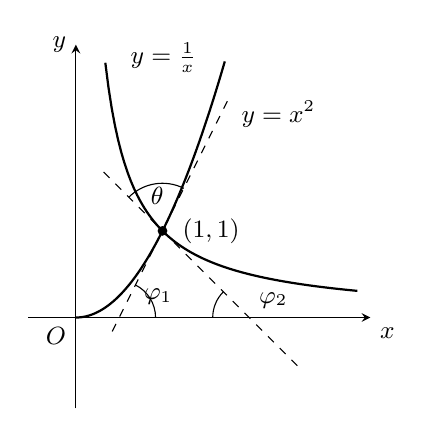
\begin{tikzpicture}[scale=1.1,>=stealth,font=\small]
  \draw[->] (-0.55,0) -- (3.40,0) node[below right] {$x$};
  \draw[->] (0,-1.05) -- (0,3.15) node[left] {$y$};
  \node[below left] at (0,0) {$O$};
  % y = x^2
  \draw[thick,domain=0:1.72,samples=60] plot (\x,{\x*\x});
  \node[right] at (1.80,2.35) {$y=x^2$};
  % y = 1/x
  \draw[thick,domain=0.34:3.25,samples=80] plot (\x,{1/\x});
  \node[right] at (0.52,3.00) {$y=\frac{1}{x}$};
  % 交点 (1,1)
  \fill (1,1) circle (1.6pt);
  \node[right] at (1.12,1.00) {$(1,1)$};
  % 切线 y=2x-1 (切于 y=x^2), 交 x 轴于 (0.5,0)
  \draw[dashed] (0.42,-0.16) -- (1.75,2.50);
  % 切线 y=-x+2 (切于 y=1/x), 交 x 轴于 (2,0)
  \draw[dashed] (0.32,1.68) -- (2.62,-0.62);
  % 夹角 theta (两切线之间)
  \draw (1,1) ++(63.4:0.55) arc (63.4:135:0.55);
  \node at (0.94,1.40) {$\theta$};
  % 角 phi_1 (y=x^2 的切线与 x 轴)
  \draw (0.5,0) ++(0.42,0) arc (0:63.4:0.42);
  \node at (0.95,0.24) {$\varphi_1$};
  % 角 phi_2 (y=1/x 的切线与 x 轴)
  \draw (2,0) ++(-0.42,0) arc (180:135:0.42);
  \node at (2.28,0.20) {$\varphi_2$};
\end{tikzpicture}
\caption{}\label{fig:3.1.2}
\end{figure}

\begin{example}\label{ex:3.1.15}
质点作直线运动, 它离原点 $O$ 的位移为 $x(t)$, 求质点运动的加速度(速度的变化率). 进而问: 在高度为 $h_0$ 处的物体作自由落体运动, 何时落到地面?
\end{example}

\begin{solution}
由例~\ref{ex:3.1.1} 知, (瞬时)速度 $v(t) = x'(t) = \lim\limits_{\Delta t\to0}\frac{x(t+\Delta t) - x(t)}{\Delta t}$, 它是质点位移 $x(t)$ 对时间 $t$ 的导数. 如果极限
\[
a(t) = v'(t) = \lim_{\Delta t\to0}\frac{v(t+\Delta t) - v(t)}{\Delta t} = \lim_{\Delta t\to0}\frac{x'(t+\Delta t) - x'(t)}{\Delta t} \xlongequal{\text{记作}} x''(t)
\]
存在且有限, 则称它为质点运动的加速度, 它是速度 $v(t)$ 对 $t$ 的导数, 也是位移 $x(t)$ 的 $2$ 阶导数.

自由落体运动, 其离地面高度 $h(t) = h_0 - \frac{1}{2}gt^2$, 速度 $v(t) = h'(t) = -gt$, 加速度 $a(t) = v'(t) = h''(t) = -g\ (\approx 980\,\text{cm/s}^2)$, 它是匀加速运动. 当 $t = \sqrt{\frac{2h_0}{g}}$ 时, 物体下落到地面.
\end{solution}

\begin{example}\label{ex:3.1.16}
汽车前灯的反光镜(或探照灯, 如图~\ref{fig:3.1.3} 所示)是由抛物线绕对称轴旋转而成的旋转抛物面. 这种反光镜就是利用抛物线的光学特性: 若光源置于抛物线的焦点上, 则光线经抛物线反射成一束平行于对称轴的光线(如图~\ref{fig:3.1.4} 所示). 试证之.
\end{example}

\begin{figure}[htbp]
\centering
\begin{minipage}[t]{0.45\textwidth}
\centering
\begin{tikzpicture}[scale=0.9,>=stealth]
  % 抛物面(旋转抛物面的轴截面)
  \draw[thick,domain=0.10:2.30,samples=80,smooth,variable=\t]
    plot ({0.18+1.67*((\t-1.20)/1.10)*((\t-1.20)/1.10)}, {\t});
  % 开口(椭圆, 后半虚线)
  \draw[thick] (1.85,2.30) arc (90:-90:0.30 and 1.10);
  \draw[dashed] (1.85,2.30) arc (90:270:0.30 and 1.10);
  % 焦点 F
  \draw[dashed] (0.62,1.20) circle (0.18);
  \fill (0.62,1.20) circle (1.4pt);
  \node[left,font=\small] at (0.42,1.20) {$F$};
  % 自焦点发出的光线经抛物面反射后平行于对称轴射出
  \foreach \y/\xb in {0.32/1.249,0.58/0.710,0.86/0.339,1.54/0.339,1.82/0.710,2.08/1.249}{
    \draw[->] (0.62,1.20) -- (\xb,\y);
    \draw[->] (\xb,\y) -- (2.75,\y);
  }
  \draw[->] (0.62,1.20) -- (2.75,1.20);
  \node[below,font=\small] at (1.45,-0.05) {探照灯};
\end{tikzpicture}
\caption{}\label{fig:3.1.3}
\end{minipage}
\hfill
\begin{minipage}[t]{0.45\textwidth}
\centering
\begin{tikzpicture}[scale=0.9,>=stealth]
  \draw[thick,domain=0.10:2.30,samples=80,smooth,variable=\t]
    plot ({0.18+1.67*((\t-1.20)/1.10)*((\t-1.20)/1.10)}, {\t});
  \draw[thick] (1.85,2.30) arc (90:-90:0.30 and 1.10);
  \draw[dashed] (1.85,2.30) arc (90:270:0.30 and 1.10);
  \draw[dashed] (0.62,1.20) circle (0.18);
  \fill (0.62,1.20) circle (1.4pt);
  \node[left,font=\small] at (0.42,1.20) {$F$};
  % 平行于对称轴的入射光线经抛物面反射后汇聚于焦点
  \foreach \y/\xb in {0.32/1.249,0.58/0.710,0.86/0.339,1.54/0.339,1.82/0.710,2.08/1.249}{
    \draw[->] (2.75,\y) -- (\xb,\y);
    \draw[->] (\xb,\y) -- (0.62,1.20);
  }
  \draw[->] (2.75,1.20) -- (0.62,1.20);
  \node[below,font=\small] at (1.45,-0.05) {太阳灶};
\end{tikzpicture}
\caption{}\label{fig:3.1.4}
\end{minipage}
\end{figure}

\begin{proof}
设抛物线的方程为 $y^2 = 2px$, 则焦点为 $F\left(\frac{p}{2}, 0\right)$. 在抛物线上任取一点 $A(x_0, y_0)$, 过 $A$ 点作切线 $L$, 记 $L$ 与线段 $AF$ 的夹角为 $\alpha$, $L$ 与 $x$ 轴的夹角为 $\beta$. 根据光学原理: 光线的入射角等于反射角. 因此, 如果能证明 $\alpha = \beta$, 则就证明了反射光线平行于 $x$ 轴(对称轴). 记 $L$ 与 $x$ 轴的交点为 $B$. 于是, $\alpha = \beta \iff AF = BF$.

将 $y^2 = 2px$ 两边关于 $x$ 求导得 $2yy' = 2p$, 所以, $y' = \frac{p}{y}$. 因此, 抛物线 $y^2 = 2px$ 在点 $A(x_0, y_0)$ 的切线 $L$ 的斜率为 $y'|_{x=x_0} = \frac{p}{y_0}$, 故 $L$ 的方程为
\[
y - y_0 = \frac{p}{y_0}(x - x_0).
\]
在上式中, 令 $y = 0$, 即得 $B$ 点坐标为 $(-x_0, 0)$. 因此,
\[
BF = \left|\frac{p}{2} + x_0\right|,
\]
\[
AF = \sqrt{\left(x_0 - \frac{p}{2}\right)^2 + y_0^2} = \sqrt{\left(x_0 - \frac{p}{2}\right)^2 + 2px_0} = \left|\frac{p}{2} + x_0\right| = BF.
\]
根据上述数学原理, 如果有一束平行于 $x$ 轴的光线经旋转抛物面反射到抛物线焦点 $F$(太阳灶就是由这原理造出来的, 以致在 $F$ 处达到高温, 如图~\ref{fig:3.1.5} 所示).
\end{proof}

\begin{figure}[htbp]
\centering
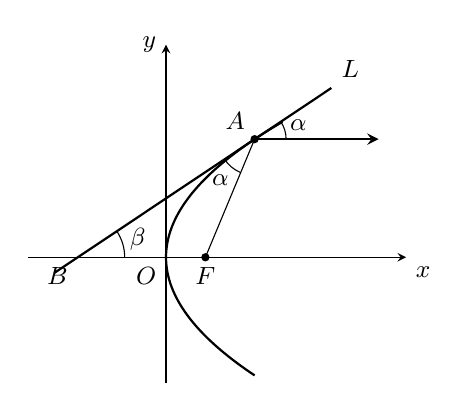
\begin{tikzpicture}[scale=1.0,>=stealth,font=\small]
  \draw[->] (-1.75,0) -- (3.05,0) node[below right] {$x$};
  \draw[->] (0,-1.60) -- (0,2.70) node[left] {$y$};
  \node[below left] at (0,0) {$O$};
  % 抛物线 y^2 = 2x  =>  x = y^2/2
  \draw[thick,domain=-1.50:1.72,samples=80,smooth,variable=\t] plot ({0.5*\t*\t},{\t});
  \coordinate (A) at (1.125,1.5);
  \coordinate (B) at (-1.125,0);
  \coordinate (F) at (0.5,0);
  % 切线 L (过 A, B)
  \draw[thick] (-1.42,-0.20) -- (2.10,2.15) node[above right] {$L$};
  % 反射光线 (平行于 x 轴)
  \draw[->,thick] (A) -- (2.70,1.5);
  % 焦半径 AF
  \draw (A) -- (F);
  \fill (A) circle (1.5pt);
  \node[above left] at (A) {$A$};
  \fill (F) circle (1.5pt);
  \node[below] at (F) {$F$};
  \node[below left] at (B) {$B$};
  % 角 beta (B 处: L 与 x 轴)
  \draw (B) ++(0.60,0) arc (0:33.7:0.60);
  \node at (-0.36,0.23) {$\beta$};
  % 角 alpha (A 处: L 与反射光线)
  \draw (A) ++(0.40,0) arc (0:33.7:0.40);
  \node at (1.68,1.68) {$\alpha$};
  % 角 alpha (A 处: L 与 AF)
  \draw (A) ++(213.7:0.46) arc (213.7:247.4:0.46);
  \node at (0.69,0.98) {$\alpha$};
\end{tikzpicture}
\caption{}\label{fig:3.1.5}
\end{figure}

\begin{exblock}{练习题 3.1}
  \item 设函数 $f$ 在点 $x_0$ 处可导, 则 $\lim\limits_{\Delta x\to0}\frac{f(x_0+\Delta x) - f(x_0-\Delta x)}{\Delta x} = 2f'(x_0)$. 举例说明: 即使上式左边的极限存在且有限, $f$ 在点 $x_0$ 处也未必可导.

  \item 在抛物线 $y = x^2$ 上哪些点的切线满足下面条件:
  \begin{enumerate}[label=(\arabic*)]
    \item 平行于直线 $y = 4x - 5$;
    \item 垂直于直线 $2x - 6y + 5 = 0$;
    \item 与直线 $3x - y + 1 = 0$ 交成 $45^\circ$ 的角.
  \end{enumerate}

  \item 证明: 抛物线 $y = x^2$ 上的两点 $(x_1, x_1^2)$ 与 $(x_2, x_2^2)$ 处的切线互相垂直的充分必要条件是 $x_1$ 与 $x_2$ 适合关系 $4x_1x_2 + 1 = 0$.

  \item 设 $f(x) = x(x-1)^2(x-2)^3$. 求 $f'(0)$, $f'(1)$, $f'(2)$.

  \item 设 $f(x_0) = 0$, $f'(x_0) = 4$. 求极限 $\lim\limits_{\Delta x\to0}\frac{f(x_0+\Delta x)}{\Delta x}$.

  \item 确定曲线 $y = \ln x$ 上哪些点的切线平行于下列直线: (1) $y = x - 1$; (2) $y = 2x - 3$.

  \item 求下列曲线在指定点 $P$ 的切线方程与法线方程:
  \begin{enumerate}[label=(\arabic*)]
    \item $y = \frac{x^2}{4}$, $P = (2,1)$;
    \item $y = \cos x$, $P = (0,1)$.
  \end{enumerate}

  \item 求下列函数的导函数:
  \begin{enumerate}[label=(\arabic*)]
    \item $f(x) = |x|^3$;
    \item $f(x) = \begin{cases}x+1, & x \geqslant 0,\\ 1, & x < 0.\end{cases}$
  \end{enumerate}

  \item 设 $f(x) = \begin{cases}x^2, & x \geqslant 3,\\ ax+b, & x < 3.\end{cases}$ 试确定 $a$, $b$ 的值, 使 $f$ 在 $x=3$ 处可导.

  \item 设 $g(0) = g'(0) = 0$, $f(x) = \begin{cases}g(x)\sin\frac{1}{x}, & x \neq 0,\\ 0, & x = 0.\end{cases}$ 求 $f'(0)$.

  \item 设函数 $f$ 在点 $x_0$ 处存在左右导数. 证明: $f$ 在点 $x_0$ 处连续.

  \item 设函数 $f$ 在 $[a,b]$ 上连续, 且 $f(a) = f(b) = K$, $f'_+(a)\cdot f'_-(b) > 0$. 证明: 在 $(a,b)$ 内至少有一点 $\xi$, 使 $f(\xi) = K$.

  \item 设 $f$ 在 $\mathbb{R}$ 上可导, 并且 $\lim\limits_{x\to\infty}f(x) = a \in \mathbb{R}$. 证明: 必 $\exists \xi \in \mathbb{R}$, s.t. $f'(\xi) = 0$.

  \item 设函数 $f$ 在 $x = a$ 处可导, 且 $f(a) \neq 0$. 求数列极限
  \[
  \lim_{n\to+\infty}\left(\frac{f\left(a+\frac{1}{n}\right)}{f(a)}\right)^n.
\]

  \item 设函数 $\varphi$ 在点 $a$ 处连续, 又在 $a$ 的近旁有 $f(x) = (x-a)\varphi(x)$ 和 $g(x) = |x-a|\varphi(x)$. 证明: $f$ 在点 $a$ 处可导, 并求 $f'(a)$. 问在什么条件下 $g$ 在点 $a$ 处可导.

  \item 求下列函数在指定点的导数:
  \begin{enumerate}[label=(\arabic*)]
    \item $f(x) = 3x^4 + 2x^3 + 5$, 求 $f'(0)$, $f'(1)$;
    \item $f(x) = \frac{x}{\cos x}$, 求 $f'(0)$, $f'(\pi)$;
    \item $f(x) = \sqrt{1 + \sqrt{x}}$, 求 $f'(0)$, $f'(1)$, $f'(4)$.
  \end{enumerate}

  \item 求下列函数的导数:
  \begin{enumerate}[label=(\arabic*)]
    \item $y = x^3 - 2x - 6$;
    \item $y = \sqrt{x} - \frac{1}{x}$;
    \item $y = \frac{1-x^2}{1+x+x^2}$;
    \item $y = \frac{x}{m} + \frac{m}{x} + 2\sqrt{x} + \frac{2}{\sqrt{x}}$;
    \item $y = x^3\log_3 x$;
    \item $y = \mathrm{e}^x\cos x$;
    \item $y = (x^2+1)(3x-1)(1-x^3)$;
    \item $y = \frac{\tan x}{x}$;
    \item $y = \frac{1+\ln x}{1-\ln x}$;
    \item $y = (\sqrt{x}+1)\arctan x$;
    \item $y = \frac{1+x^2}{\sin x + \cos x}$;
    \item $y = \mathrm{e}^{ax}\cos bx$;
    \item $y = \frac{\cos x - \sin x}{\cos x + \sin x}$;
    \item $y = x\sin x\ln x$;
    \item $y = \sqrt{x + \sqrt{x + \sqrt{x}}}$;
    \item $y = \ln(\cos x + \sin x)$;
    \item $y = (x^2-1)^3$;
    \item $y = \left(\frac{1+x^2}{1-x}\right)^3$;
    \item $y = \ln(\ln x)$;
    \item $y = \ln\frac{\sqrt{1+x} - \sqrt{1-x}}{\sqrt{1+x} + \sqrt{1-x}}$;
    \item $y = (\arctan x^3)^2$;
    \item $y = \arcsin(\sin^2 x)$;
    \item $y = \sin(\sin(\sin x))$;
    \item $y = \sin\left(\frac{x}{\sin\left(\frac{x}{\sin x}\right)}\right)$;
    \item $y = (x-a_1)^{a_1}(x-a_2)^{a_2}\cdots(x-a_n)^{a_n}$;
    \item $y = \sqrt[3]{\frac{(x+1)^2(x+2)^3}{(x+3)^4(x+4)^5}}$.
  \end{enumerate}

  \item 求下列函数的导数:
  \begin{enumerate}[label=(\arabic*)]
    \item $y = \frac{ax+b}{cx+d}$, 其中 $a, b, c, d$ 为常数;
    \item $y = \ln(x + \sqrt{x^2+a^2})$;
    \item $y = x^{x^x}$.
  \end{enumerate}

  \item 证明:
  \begin{enumerate}[label=(\arabic*)]
    \item $(\sinh x)' = \cosh x$;
    \item $(\cosh x)' = \sinh x$;
    \item $(\tanh x)' = \frac{1}{\cosh^2 x}$;
    \item $(\coth x)' = \frac{1}{\sinh^2 x}$.
  \end{enumerate}

  \item 以 $\operatorname{arsinh} x$, $\operatorname{arcosh} x$, $\operatorname{artanh} x$, $\operatorname{arcoth} x$ 分别表示各双曲函数的反函数. 试求下列函数的导数:
  \begin{enumerate}[label=(\arabic*)]
    \item $y = \operatorname{arsinh} x$;
    \item $y = \operatorname{arcosh} x$;
    \item $y = \operatorname{artanh} x$;
    \item $y = \operatorname{arcoth} x$.
  \end{enumerate}

  \item 设 $g$ 可导, $a$ 为实数. 对下列各函数计算 $f'(x)$, $f'(x+1)$, $f'(x-1)$:
  \begin{enumerate}[label=(\arabic*)]
    \item $f(x) = x^3$;
    \item $f(x) = g(x + g(x))$;
    \item $f(x) = g(x)g(a)$;
    \item $f(x) = g(x)g(x)$.
  \end{enumerate}

  \item 设 $f$ 为可导函数. 证明: 若 $x=1$ 时, 有 $\frac{\mathrm{d}}{\mathrm{d}x}f(x^2) = \frac{\mathrm{d}}{\mathrm{d}x}f^2(x)$, 且必有 $f'(1) = 0$ 或 $f(1) = 1$.

  \item 利用 $1 + x + \cdots + x^n$ 的和, 求出下列各式的和:
  \begin{enumerate}[label=(\arabic*)]
    \item $1 + 2x + 3x^2 + \cdots + nx^{n-1}$;
    \item $\sum\limits_{k=1}^{n}\frac{k}{2^{k-1}}$;
    \item $1^2 + 2^2 x + 3^2 x^2 + \cdots + n^2 x^{n-1}$.
  \end{enumerate}

  \item 设 $f$ 为可导函数, 求下列各函数的一阶导数:
  \begin{enumerate}[label=(\arabic*)]
    \item $y = f(\mathrm{e}^x)\mathrm{e}^{f(x)}$;
    \item $y = f(f(f(x)))$.
  \end{enumerate}

  \item 设 $\varphi$, $\psi$ 为可导函数, 求 $y'$:
  \begin{enumerate}[label=(\arabic*)]
    \item $y = \sqrt{\varphi^2(x) + \psi^2(x)}$;
    \item $y = \arctan\frac{\varphi(x)}{\psi(x)}$;
    \item $y = \log_{\varphi(x)}\psi(x)$ ($\varphi(x) > 0$, $\varphi(x) \neq 1$, $\psi(x) > 0$).
  \end{enumerate}

  \item 在曲线 $y = x^3$ 上取一点 $P$, 过 $P$ 的切线与该曲线交于 $Q$. 证明: 曲线在 $Q$ 点处的切线斜率正好是在 $P$ 点处切线斜率的 $4$ 倍.

  \item 设有一吊桥, 其铁链成抛物线型, 两端系于相距 $100$ m 高度相同的支柱上, 铁链的最低点在悬点下 $10$ m 处, 求铁链与支柱所成的角.

  \item 证明: 双曲线 $xy = a > 0$ 在各点处的切线与两坐标轴所围成的三角形的面积为常数.

  \item 有一底半径为 $R$ cm, 高为 $h$ cm 的正圆锥容器, 顶点有一小孔, 以便向容器内注水. 今以 $A\ \text{cm}^3/\text{s}$ 的速度向容器内注水, 试求容器内水位等于锥高一半时, 水面上升的速度.

  \item 水自高为 $18$ cm、底半径为 $6$ cm 的圆锥形漏斗流入直径为 $10$ cm 的圆柱形桶内. 已知漏斗水深 $12$ cm 时水面下降速度为 $1$ cm/s, 求此时桶中水面上升的速度.
\end{exblock}

\begin{exblock}{思考题 3.1}
  \item 证明: Riemann 函数 $R(x)$ 处处不可导.

  \item 构造一个可导函数 $f$, 使 $f$ 在有理点处取有理数值, 它的导函数在有理点处取无理数值.

  \item
  \begin{enumerate}[label=(\arabic*)]
    \item 构造一个连续函数, 它仅在已知点 $a_1, \cdots, a_n$ 处不可导;
    \item 构造一个函数, 它仅在点 $a_1, \cdots, a_n$ 处可导.
  \end{enumerate}

  \item 设 $f$ 为三次多项式, 且 $f(a) = f(b) = 0$. 证明: 函数 $f$ 在 $[a,b]$ 上不变号的必要充分条件是 $f'(a)f'(b) \leqslant 0$.

  \item 证明组合恒等式:
  \begin{enumerate}[label=(\arabic*)]
    \item $\sum\limits_{k=1}^{n}kC_n^k = n2^{n-1}$, $n \in \mathbb{N}$;
    \item $\sum\limits_{k=1}^{n}k^2C_n^k = n(n+1)2^{n-2}$, $n \in \mathbb{N}$.
  \end{enumerate}
  (提示: 分别对 $(1+x)^n = \sum\limits_{k=0}^{n}C_n^k x^k$ 与 $nx(1+x)^{n-1} = \sum\limits_{k=1}^{n}kC_n^k x^{k-1}$ 两边关于 $x$ 求导.)

  \item 设 $f(0) = 0$, $f'(0)$ 存在且有限, 令 $x_n = f\left(\frac{1}{n^2}\right) + f\left(\frac{2}{n^2}\right) + \cdots + f\left(\frac{n}{n^2}\right)$. 证明: $\lim\limits_{n\to+\infty}x_n = \frac{f'(0)}{2}$. 并利用以上结果计算:
  \begin{enumerate}[label=(\arabic*)]
    \item $\lim\limits_{n\to+\infty}\sum\limits_{k=1}^{n}\sin\frac{k}{n^2}$;
    \item $\lim\limits_{n\to+\infty}\prod\limits_{k=1}^{n}\left(1 + \frac{k}{n^2}\right)$, 其中 $\prod\limits_{k=1}^{n}$ 表示 $n$ 个数连乘.
  \end{enumerate}

  \item 设函数 $f$ 在 $x=0$ 处连续, 如果 $\lim\limits_{x\to0}\frac{f(2x) - f(x)}{x} = m$, 证明: $f'(0) = m$.

  \item 在区间 $[-1,1]$ 上讨论二次函数 $f(x) = ax^2 + bx + c$, 如果 $|f(x)| \leqslant 1$, $\forall x \in [-1,1]$, 证明: $|f'(x)| \leqslant 4$, $\forall x \in [-1,1]$.

  \item (1) 设 $f_n$, $f$ 为 $\mathbb{R}$ 上的一元函数, $f_n$ 在 $\mathbb{R}$ 上连续, $n = 1, 2, \cdots$, 且 $\lim\limits_{n\to+\infty}f_n(x) = f(x)$, $x \in \mathbb{R}$. 证明: 存在 $(\alpha,\beta) \subset \mathbb{R}$, 使得 $f$ 在 $(\alpha,\beta)$ 上是有界的.
  (2) 设 $g$ 在 $\mathbb{R}$ 上可导. 证明: 存在 $(\alpha,\beta) \subset \mathbb{R}$, 使得 $g'$ 在 $(\alpha,\beta)$ 上有界.
  (3) 使得导函数 $g'$ 在任何开区间 $(\alpha,\beta) \subset \mathbb{R}$ 上都无界的函数 $g$ 是不存在的.

  \item 在 $[0,1]$ 上适合条件 $|P| \leqslant 1$ 的二次多项式 $P$ 的全体记为 $V$, 求 $\sup\{|P'(0)|\}$.
\end{exblock}
